\documentclass[aspectratio=169]{beamer}


%%% PAQUETES  %%%
%%% PAQUETES  %%%

%%% Soporte extendido de colores
\usepackage{xcolor}
    % Definiciones colores extra
    %% Ref: http://latexcolor.com/
    \definecolor{coolblack}{rgb}{0.0, 0.18, 0.39}
    \definecolor{dimgray}{rgb}{0.41, 0.41, 0.41}

%%% Paquete para poner hipervinculos más finos \href
\PassOptionsToPackage{hyphens}{url}
\usepackage{hyperref}

   %Colores personalizados
    \hypersetup{
        colorlinks=true,
        linkcolor=black,
        filecolor=black,
        %%% Necesita su propia definicion de color
        citecolor=dimgray,
        urlcolor=coolblack,
    }

%%% Formato y tipografía de URL, direcciones de correo...
\usepackage{url}
    \def\UrlFont{\rmfamily}

%%% Usados por graficas de barras
\usepackage{textcomp}
\usepackage{tikz}
\usepackage{pgfplots}
\usepackage{pgfplotstable} 
\usepackage{csvsimple}% Generates table from .csv
\pgfplotsset{compat=1.7}
\usepackage{subcaption}
\usepgfplotslibrary{groupplots}

% PGFPlots Settings
\pgfplotsset{
SmallBarPlot/.style={
    font=\footnotesize,
    ybar,
    width=\linewidth,
    ymin=0,
    xtick=data,
    xticklabel style={text width=1.5cm, rotate=90, align=center}
},
BlueBars/.style={fill=blue!20, bar width=0.25},
RedBars/.style={fill=red!20, bar width=0.25},
GreenBars/.style={fill=green!20, bar width=0.25}
}

%% Para incluir en el texto o en el pie de la figura la leyenda con colores.
\DeclareRobustCommand\legendbox[1]{(\textcolor{#1}{#1 bars}~\begin{tikzpicture}[x=0.2cm, y=0.2cm] \draw [color=black, fill=#1!20] (0,0) -- (0,1) -- (0.6,1) -- (0.6,0) -- (0, 0); \end{tikzpicture})}

\usepackage{booktabs} % usado en tablas generadas con JASP


%%%%%%%%%%%%%%%%%%%%%%%%%%%%%%% HEREDADOS JNIC %%%%%%%%%%%%%%%%%%%%%%%%%%%%%%%

%%% TODO NOTES y definición 2cm de margen para que no se solapen añadido colores comentarios
 \setlength {\marginparwidth }{2cm} 
 \usepackage{todonotes}
 \usepackage[normalem]{ulem}

%%% Paquete para comentarios
\usepackage{verbatim}

%%% Tildes y demás caracteres en castellano...
%\usepackage[latin1]{inputenc}
% o bien
\usepackage[utf8]{inputenc}

%%% Fuente Times...
\usepackage{times}

%%% Figuras en formato .png, .ps, pdf o eps
\usepackage{graphicx}
%%\usepackage{subfigure}
\DeclareGraphicsExtensions{.png,.eps,.ps,.pdf}

%%% Soporte graficos svg
\usepackage{svg}

%%% Sección para definir explícitamente la separación de sílabas al final de una línea:
\hyphenation{si-guien-do}

%%% Secciones etc. en castellano
%\usepackage[spanish,es-tabla]{babel}

%%% Secciones etc. en Ingles
\usepackage[english]{babel}


%%% Paquete para usar simbolos y scripts de dibujado
\usepackage{tikz}
\def\checkmark{\tikz\fill[scale=0.4](0,.35) -- (.25,0) -- (1,.7) -- (.25,.15) -- cycle;} 
\usetikzlibrary{shapes,arrows}

% Define Block styles
\tikzstyle{decisionBL} = [diamond, draw, fill=blue!20,text width=10em, text badly centered, node distance=3cm, inner sep=0pt]
\tikzstyle{blockBL} = [rectangle, draw, fill=blue!20,text width=9em, text centered, rounded corners, minimum height=4em]
\tikzstyle{blockYL} = [rectangle, draw, fill=yellow!20, text width=9em, text centered, rounded corners, minimum height=4em]
\tikzstyle{blockGR} = [rectangle, draw, fill=green!20, text width=9em, text centered, rounded corners, minimum height=4em]
\tikzstyle{blockRD} = [rectangle, draw, fill=red!20, text width=9em, text centered, rounded corners, minimum height=4em]
\tikzstyle{blockWH} = [rectangle, draw, fill=white!20, text width=9em, text centered, rounded corners, minimum height=4em]
\tikzstyle{line} = [draw, -latex']
\tikzstyle{cloud} = [draw, ellipse,fill=red!20, node distance=4.5cm,minimum height=4em]

%%% Para usar ficheros tex de infografias Inkscape
\usepackage{pstricks}
%\definecolor{Azuloscuro-cisis}{RGB}{1,62,133}
\definecolor{Azulclaro-cisis}{RGB}{0,101,219}

\definecolor{LUCopper}{rgb}{0.8,0,0} %títulos slides
\definecolor{LUBlue}{rgb}{0.07, 0.04, 0.56}

\definecolor{LUPink}{rgb}{0.24,0.82,0.44}
\definecolor{LUGreen}{rgb}{0.24,0.82,0.44}
\definecolor{LUWhite}{rgb}{1,1,1} % fondo
%%% COMANDOS  %%%
%%% COMANDOS  %%%

%%% A cursiva  %%%
\newcommand{\cursiva}[1]{\em{#1}}


%%% Fuzzing en bonito  %%%
\newcommand{\fz}{\em fuzzing}

%%% Atajos estilo  %%%

\newcommand{\CLASSINPUTinnersidemargin}{18mm}
\newcommand{\CLASSINPUToutersidemargin}{12mm}
\newcommand{\CLASSINPUTtoptextmargin}{20mm}
\newcommand{\CLASSINPUTbottomtextmargin}{25mm}

\newcommand{\new}[1]{\textcolor{olive}{{#1}}}
%\newcommand{\old}[1]{\textcolor{purple}{{\sout{#1}}}}
\newcommand{\wip}[1]{\textcolor{blue}{{#1}}}
%\newcommand{\checkthis}[1]{\textcolor{orange}{{#1}}}
\newcommand{\diego}[1]{\textcolor{magenta}{{#1}}}
\newcommand{\vmodixit}[1]{\textcolor{teal}{{#1}}}

\newcommand{\old}[1]{\textcolor{purple}{{\sout{#1}}}}
\newcommand{\camino}[1]{\textcolor{olive}{{#1}}}
\newcommand{\fjrodl}[1]{\textcolor{blue}{{#1}}}
\newcommand{\checkthis}[1]{\textcolor{orange}{{#1}}}

%%% Entornos  %%%
\newcounter{definicion}
\newenvironment{definicion}[1]{%
    \refstepcounter{definicion}\par\medskip%
    \noindent \textbf{Definición~\thedefinicion. #1}.\ %
}{\medskip}

%%%% Soporte para el logo de ORCID
%\newcommand{\orcid}[1]{\href{https://orcid.org/#1}{\textcolor[HTML]{A6CE39}{\aiOrcid}}}



\title[{\fz} robots HPC \& LLM]{\textbf{Fuzzing Robotic Software using HPC and LLM}\\
%\tiny \\
%\tiny y desacoplada para el uso de técnicas de {\fz} en HPC.\\
\small{\underline{Francisco Borja Garnelo Del Río}, Francisco J. Rodríguez Lera } \\
\small{Camino Fernández Llamas, Vicente Matellán Olivera} \\
\tiny{Universidad de León - 
Campus de Vegazana s/n, 24071 León (Spain)} \\
\tiny{infbgd01@estudiantes.unileon.es, \{fjrodl, cferll, vmato\}@unileon.es}
}

\titlecolor{LUWhite} % Choose between LUPink, LULBlue, LUIvory, LUGreen


% Titulo como imagen conferencia2024.png
%        Computational Intelligence in Security for Information Systems
%            17th International conference 9-11 October 2024

\titleimage{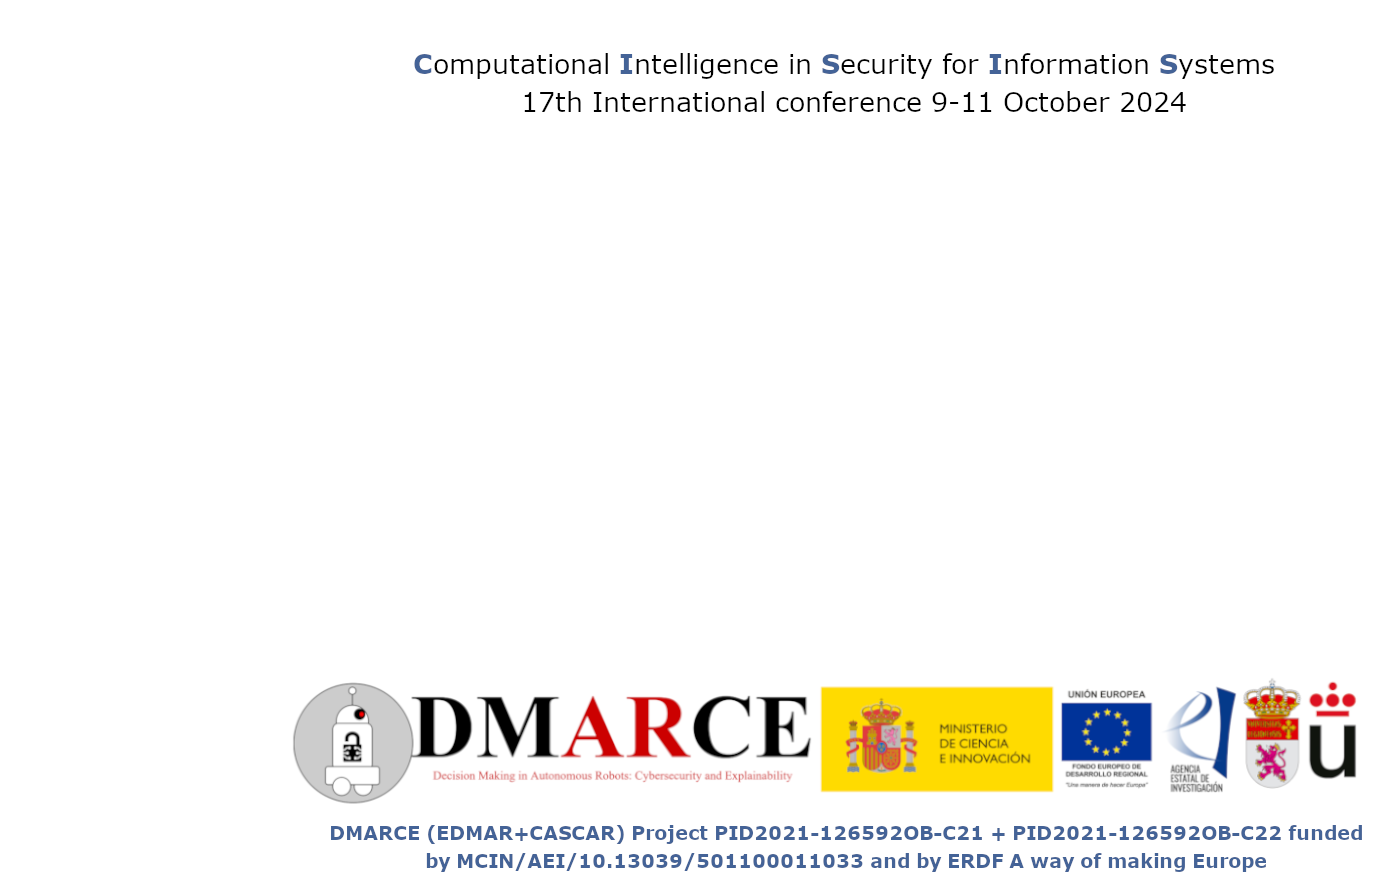
\includegraphics[scale=0.55]{./img/conferencia2024_logos.png}}

\author{Francisco B. Garnelo del Río (infbgd01@estudiantes.unileon.es)}

%\subtitle{\\ 
%\small{\underline{\\Francisco Borja Garnelo Del Río}, \\Francisco J. Rodríguez Lera,}\\ 
%\small{Camino Fernández Llamas, Vicente Matellán Olivera} \\
%\tiny{Universidad de León - Campus de Vegazana s/n, 24071 León (Spain)} \\
%\tiny{infbgd01@estudiantes.unileon.es, \{fjrodl, cferll, vmato\}@unileon.es}
%} 

\date{CISIS 2024}

\begin{document}
%\renewcommand{\contentsname}{Contenidos}
%\renewcommand{\figurename}{Figura}
%\renewcommand{\tablename}{Tabla}
%\renewcommand{\sectionname}{Sección}
%\renewcommand{\subsectionname}{Subsección}
%\renewcommand{\partname}{Parte}

%% TODO: Actualizar tabla una vez cerrada estructura.

\titleframe
 \begin{frame}{Table of Contents}
\begin{enumerate}
\item Introduction
\begin{itemize}
%    \item Concepts
    \item Challenges \& innovativation
%    \item Framework \& key
    \item Research Objectives
    \item Goals \& Hypotheses
\end{itemize}
\item Materials and Methods
\begin{itemize}
    \item Infrastructures
    \item Software
\end{itemize}
\item Proof-of-Concept Design
\begin{itemize}
    \item Simulation
    \item Integration
    \item Validation    
\end{itemize}    
\item Contribution
\item Conclusions and Future Work
\end{enumerate}
 \end{frame}

 %% REF: Cajas https://texdoc.org/serve/tcolorbox.pdf/0

 % INTRODUCCION %%%%%%%%%%%%%%%%%%%%%%%%%%%%%%%%%%%%%%%%%%%%%%%%%
\begin{comment}  
\section{Introduction}
%\frame{\sectionpage}
\begin{frame}{Introduction}

 
  \only<1>{
    
\begin{tcolorbox}[drop shadow southeast,
enhanced,colback=blue!5!white,colframe=Azuloscuro-cisis]
\textbf{Large Language Model (LLM)}is a type of artificial intelligence designed to understand and generate human-like text based on vast amounts of data. It uses deep learning techniques to predict and produce coherent and contextually relevant language outputs.
\end{tcolorbox}


\begin{tcolorbox}[drop shadow southeast,
enhanced,colback=blue!5!white,colframe=Azuloscuro-cisis]
\textbf{Fuzzing} is the automation of generating and testing malformed inputs in software in order to find unexpected behavior in the software.
\end{tcolorbox}

\begin{tcolorbox}[drop shadow southeast,
enhanced,colback=blue!5!white,colframe=Azuloscuro-cisis]
\textbf{Robotic systems} are systems that interact with their environment, including people, through the use of numerous sensors, actuators, and user interfaces to give intelligent services and information.
\end{tcolorbox}

\begin{tcolorbox}[drop shadow southeast,
enhanced,colback=blue!5!white,colframe=Azuloscuro-cisis]
\textbf{High Performance Computing (HPC)} is a technique that processes huge multidimensional information and solves complex problems at incredibly fast rates by using clusters of powerful processors operating in parallel.
\end{tcolorbox}
}
\end{frame}
\end{comment}



%%% Introduction %%%%%%%%%%%%%%%
\section{Introduction}
\frame{\sectionpage}

\subsection{Challenges \& innovation}
\begin{frame}{Introduction - Challenges \& innovation}

\only<1>{

\begin{tcolorbox}[drop shadow southeast,
enhanced,colback=blue!5!white,colframe=Azuloscuro-cisis]
\textbf{Challenges in Robotic Software Testing:}
\begin{itemize}
    \item Traditional software testing methods are insufficient for complex robotic systems.
    \item Need for extensive computational resources for fuzz testing.
\end{itemize}
\end{tcolorbox}

\begin{tcolorbox}[drop shadow southeast,
enhanced,colback=blue!5!white,colframe=Azuloscuro-cisis]
\textbf{Innovative Approach:}
\begin{itemize}
    \item Development of a modular, scalable testing framework (HOUSE).
    \item Utilizing HPC for scalable and robust testing environments.
    \item AI-driven input generation for fuzz testing based on natural language commands.
\end{itemize}
\end{tcolorbox}

}

\end{frame}


%%% Research Objectives %%%%%%%%%%%%%%%
\subsection{Research Objectives}
\begin{frame}{Introduction - Research Objectives}
  \only<1>{

Main research Objectives:

\begin{tcolorbox}[drop shadow southeast,
enhanced,colback=blue!5!white,colframe=Azuloscuro-cisis]

\begin{itemize}
    \item \textbf{Strengthen Security} Apply fuzzing to enhance the security of robotic software using open-source tools within a scalable framework.
    \item \textbf{Assess AI Benefits} Investigate the benefits of integrating generative AI in the fuzzing process, focusing on message generation and mutation.
    \item \textbf{Leverage HPC Capabilities} Utilize HPC to support and scale the fuzzing process, evaluating its effectiveness based on prior studies.    
\end{itemize}

\end{tcolorbox}
}

\end{frame}



\subsection{Goals and Hypotheses}

\begin{frame}{Introduction - Goals and Hypotheses}
  \only<1>{

\begin{tcolorbox}[drop shadow southeast,
enhanced,colback=blue!5!white,colframe=Azuloscuro-cisis,title=Research question ]
How does AI contribute to the improvement of fuzzing processes in ROS2 robotic systems?
\end{tcolorbox}

This question arises from the following hypothesis and questions: 

\begin{tcolorbox}[drop shadow southeast,
enhanced,colback=blue!5!white,colframe=Azuloscuro-cisis]

\begin{itemize}
    \item \textbf{H1:} AI can significantly enhance the fuzzing process for ROS2 robotic systems.
    \item \textbf{Q1:} How does natural language simplify the definition of complex input scenarios in fuzzing?
    \item \textbf{Q2:} How does non-specialized AI hardware impact performance?    
\end{itemize}

\end{tcolorbox}
}

\end{frame}

 
\section{Materials and Methods}
\frame{\sectionpage}

%%% Framework and Tools Overview %%%%%%%%%%%%%%%
\subsection{Intro}
%\subsection{Framework and Tools}
\begin{frame}{Materials and Method - Framework \& key tools}

\only<1>{

\begin{tcolorbox}[drop shadow southeast,
enhanced,colback=blue!5!white,colframe=Azuloscuro-cisis]
\textbf{House framework Components:}
\begin{itemize}
    \item \textbf{HPC Support:} Enables large-scale testing.
    \item \textbf{Fuzzing Techniques:} Automated input generation and mutation.
    \item \textbf{AI Integration:} Natural language processing for intelligent input generation.
\end{itemize}
\end{tcolorbox}

\begin{tcolorbox}[drop shadow southeast,
enhanced,colback=blue!5!white,colframe=Azuloscuro-cisis]
\textbf{Key Tools:}
\begin{itemize}
    \item \textbf{RoboFuzz:} Core robotic fuzzing tool.
    \item \textbf{Marcoroni LLM:} AI model for generating test inputs.
    \item \textbf{Singularity:} Container technology for deployment.
\end{itemize}
\end{tcolorbox}

}

\end{frame}


%%% Concepts %%%%%%%%%%%%%%%
%\subsection{Concepts}
\begin{frame}{Materials and Methods - Concepts}
 
  \only<1>{

\begin{tcolorbox}[drop shadow southeast,
enhanced,colback=blue!5!white,colframe=Azuloscuro-cisis]
\textbf{Large Language Model (LLM)} is an AI designed to understand and generate human-like text using deep learning on vast data.
\end{tcolorbox}

\begin{tcolorbox}[drop shadow southeast,
enhanced,colback=blue!5!white,colframe=Azuloscuro-cisis]
\textbf{Fuzzing} automates the generation and testing of malformed inputs to find unexpected software behavior.
\end{tcolorbox}

\begin{tcolorbox}[drop shadow southeast,
enhanced,colback=blue!5!white,colframe=Azuloscuro-cisis]

%% REVISAR: Definicion de ROS2 framwework
%% OLD: \textbf{Robotic systems ROS2} \textbf{TODO}: Cambiar por enfoque a framework de sistema robotico.
\textbf{ROS2 framework} Provides a flexible architecture for building and deploying complex robotic systems.

\end{tcolorbox}

\begin{tcolorbox}[drop shadow southeast,
enhanced,colback=blue!5!white,colframe=Azuloscuro-cisis]
\textbf{High Performance Computing (HPC)} uses clusters of powerful processors to solve complex problems quickly.
\end{tcolorbox}


}

\end{frame}

 \subsection{Infrastructures}
%\frame{\subsectionpage}
\begin{frame}{Materials and Methods - Infrastructures}
We used two different infrastructures with \textbf{non-specialized hardware for AI}:
\begin{itemize}
    \item \textbf{Standalone} SDO,  virtual machine with 8GB ram and 6 x Intel Xeon E3-12xx v2 vcpu (virtual cpu) and linux kernel \textit{5.3.11-100.x86\_64 (x86\_64)}. Local storage on mechanical hard disks.
  
    \item \textbf{High-Performance Computing} HPC, computing cluster with Haswell nodes in bare-metal with 48GB of ram and 2 x Intel Xeon E5-2630 v3 @ 3.20GHz with a total of 16 cores and a Linux kernel \textit{3.10.0-1062.9.1.x86\_64 (x86\_64) } .
      Network storage and cache on solid disks. %The HPC manager has been used to manage the distribution of the executions, you can see in the .slurm files used the details, mainly the common HPC policy has been used to share cpu and ram resources, allowing up to 32 parallel tasks per node. 
      
\end{itemize}
\textit{NOTE: When using containers the distro is indifferent.}
\end{frame}
 
\subsection{Software}
\begin{frame}{Materials and Methods - Software}
The experiments made use of the following software:

\begin{itemize}
    \item \textbf{RoboFuzz}, an autonomous fuzz testing tool for robotic systems. 
    \item \textbf{SLURM} (Simple Linux Utility for Resource Management) a widely used open-source workload manager and job scheduler for Linux and Unix-based clusters and supercomputers.
    \item \textbf{Singularity} a container solution created to run complex applications on HPC clusters in a simple, portable, and reproducible way.
    \item \textbf{Docker}, an open container platform for developing, shipping, and running applications.
    \item \textbf{Marcoroni 7B V3-GGUF}, an auto-regressive language model designed for the English language, integrated into ROS2 using the llama\_ros package  .    
\end{itemize}

\end{frame}

%%% TODO: No logro separar esta subseccion en 3 diapositivas  
\section{Proof-of-Concept Design}
\frame{\sectionpage}
\subsection{Intro}

\begin{comment}
    

%\subsection{Open Security Testing Tools}
\begin{frame}{Proof-of-Concept Design - Open Security Testing Tools}
%%% Explanation: %%%

%Innovation and Collaboration: Open tools allow researchers to build upon each other’s work, leading to faster advancements in security testing %techniques.

%Accessibility: Students and educators can access and utilize the latest tools without financial barriers, enhancing learning and research %capabilities.

%Transparency: Open-source tools ensure that research findings can be verified and replicated, which is crucial for scientific progress.

%%% Benefits for Companies: %%%
% Enhanced Security: By using open tools, companies can identify and fix vulnerabilities more effectively, leading to more secure software.
% Cost-Effective: Open tools eliminate the need for expensive proprietary software, making security testing more affordable.
% Quality Improvement: Continuous testing and feedback loops facilitated by open tools help in developing robust and reliable software products.

\only<1>{

\textbf{Importance in Academia:}
\begin{tcolorbox}[drop shadow southeast,
enhanced,colback=blue!5!white,colframe=blue!75!black]
\begin{itemize}
    \item \textbf{Innovation and Collaboration:} Open tools foster innovation and collaboration among researchers.
    \item \textbf{Accessibility:} Provides access to cutting-edge security testing methods for educational purposes.
    \item \textbf{Transparency:} Ensures transparency and reproducibility in research.
\end{itemize}
\end{tcolorbox}

}

\only<2>{


\textbf{Benefits for Companies:}
\begin{tcolorbox}[drop shadow southeast,
enhanced,colback=blue!5!white,colframe=blue!75!black]
\begin{itemize}
    \item \textbf{Enhanced Security:} Improves software security through rigorous testing.
    \item \textbf{Cost-Effective:} Reduces costs associated with proprietary tools.
    \item \textbf{Quality Improvement:} Leads to higher quality and more reliable software products.
\end{itemize}
\end{tcolorbox}

}


\end{frame}
\end{comment}

%\subsection{Steps of fuzz testing}
\begin{frame}{Proof-of-Concept Design - Steps of fuzz testing}

 \begin{comment}
    
\begin{figure}
    \centering
    \begin{tikzpicture}[node distance=2cm, auto]
        \node (generate) [process] at (90:3cm) {\textbf{Generation} Test Data};
        \node (execute) [process] at (18:3cm) {\textbf{Simulation} Execute Tests};
        \node (monitor) [process] at (326:3cm) {\textbf{Monitor} Behavior};
        \node (analyze) [process] at (214:3cm) {\textbf{Validation} Analyze Results};
        \node (report) [process] at (162:3cm) {\textbf{Validation} Report Bugs};

        \draw [arrow] (generate) -- (execute);
        \draw [arrow] (execute) -- (monitor);
        \draw [arrow] (monitor) -- (analyze);
        \draw [arrow] (analyze) -- (report);
        \draw [arrow] (report) -- (generate);
    \end{tikzpicture}
    \caption{Fuzzing Testing Cycle Diagram}
\end{figure}
\end{comment}

\begin{figure}
    \centering
    \begin{tikzpicture}[node distance=2cm, auto]
        \node (generate) [process, fill=red!30] at (90:3cm) {1. \textbf{Generation} Test Data};
        \node (execute) [process, fill=orange!30] at (18:3cm) {2. \textbf{Simulation} Execute Tests};
        \node (monitor) [process, fill=yellow!30] at (326:3cm) {3. \textbf{Monitor} Behavior};
        \node (analyze) [process, fill=green!30] at (214:3cm) {4. \textbf{Validation} Analyze Results};
        \node (report) [process, fill=blue!30] at (162:3cm) {5. \textbf{Validation} Report Bugs};

        \draw [arrow] (generate) -- (execute);
        \draw [arrow] (execute) -- (monitor);
        \draw [arrow] (monitor) -- (analyze);
        \draw [arrow] (analyze) -- (report);
        \draw [arrow] (report) -- (generate);
    \end{tikzpicture}
    \caption{Fuzzing Testing Cycle Diagram}
\end{figure}


\end{frame}

\subsection{Generation}
\begin{frame}{Proof-of-Concept Design - Generation}
 \textbf{Integration of GenAI:} Expanded RoboFuzz's input management capabilities to utilize LLM or VLM models compatible with llama.cpp .
 %%\begin{figure*}[p!]
%\begin{figure*}[ht!]
\begin{figure}[ht!]
%%https://www.overleaf.com/learn/latex/Positioning_of_Figures
    \centerline{
    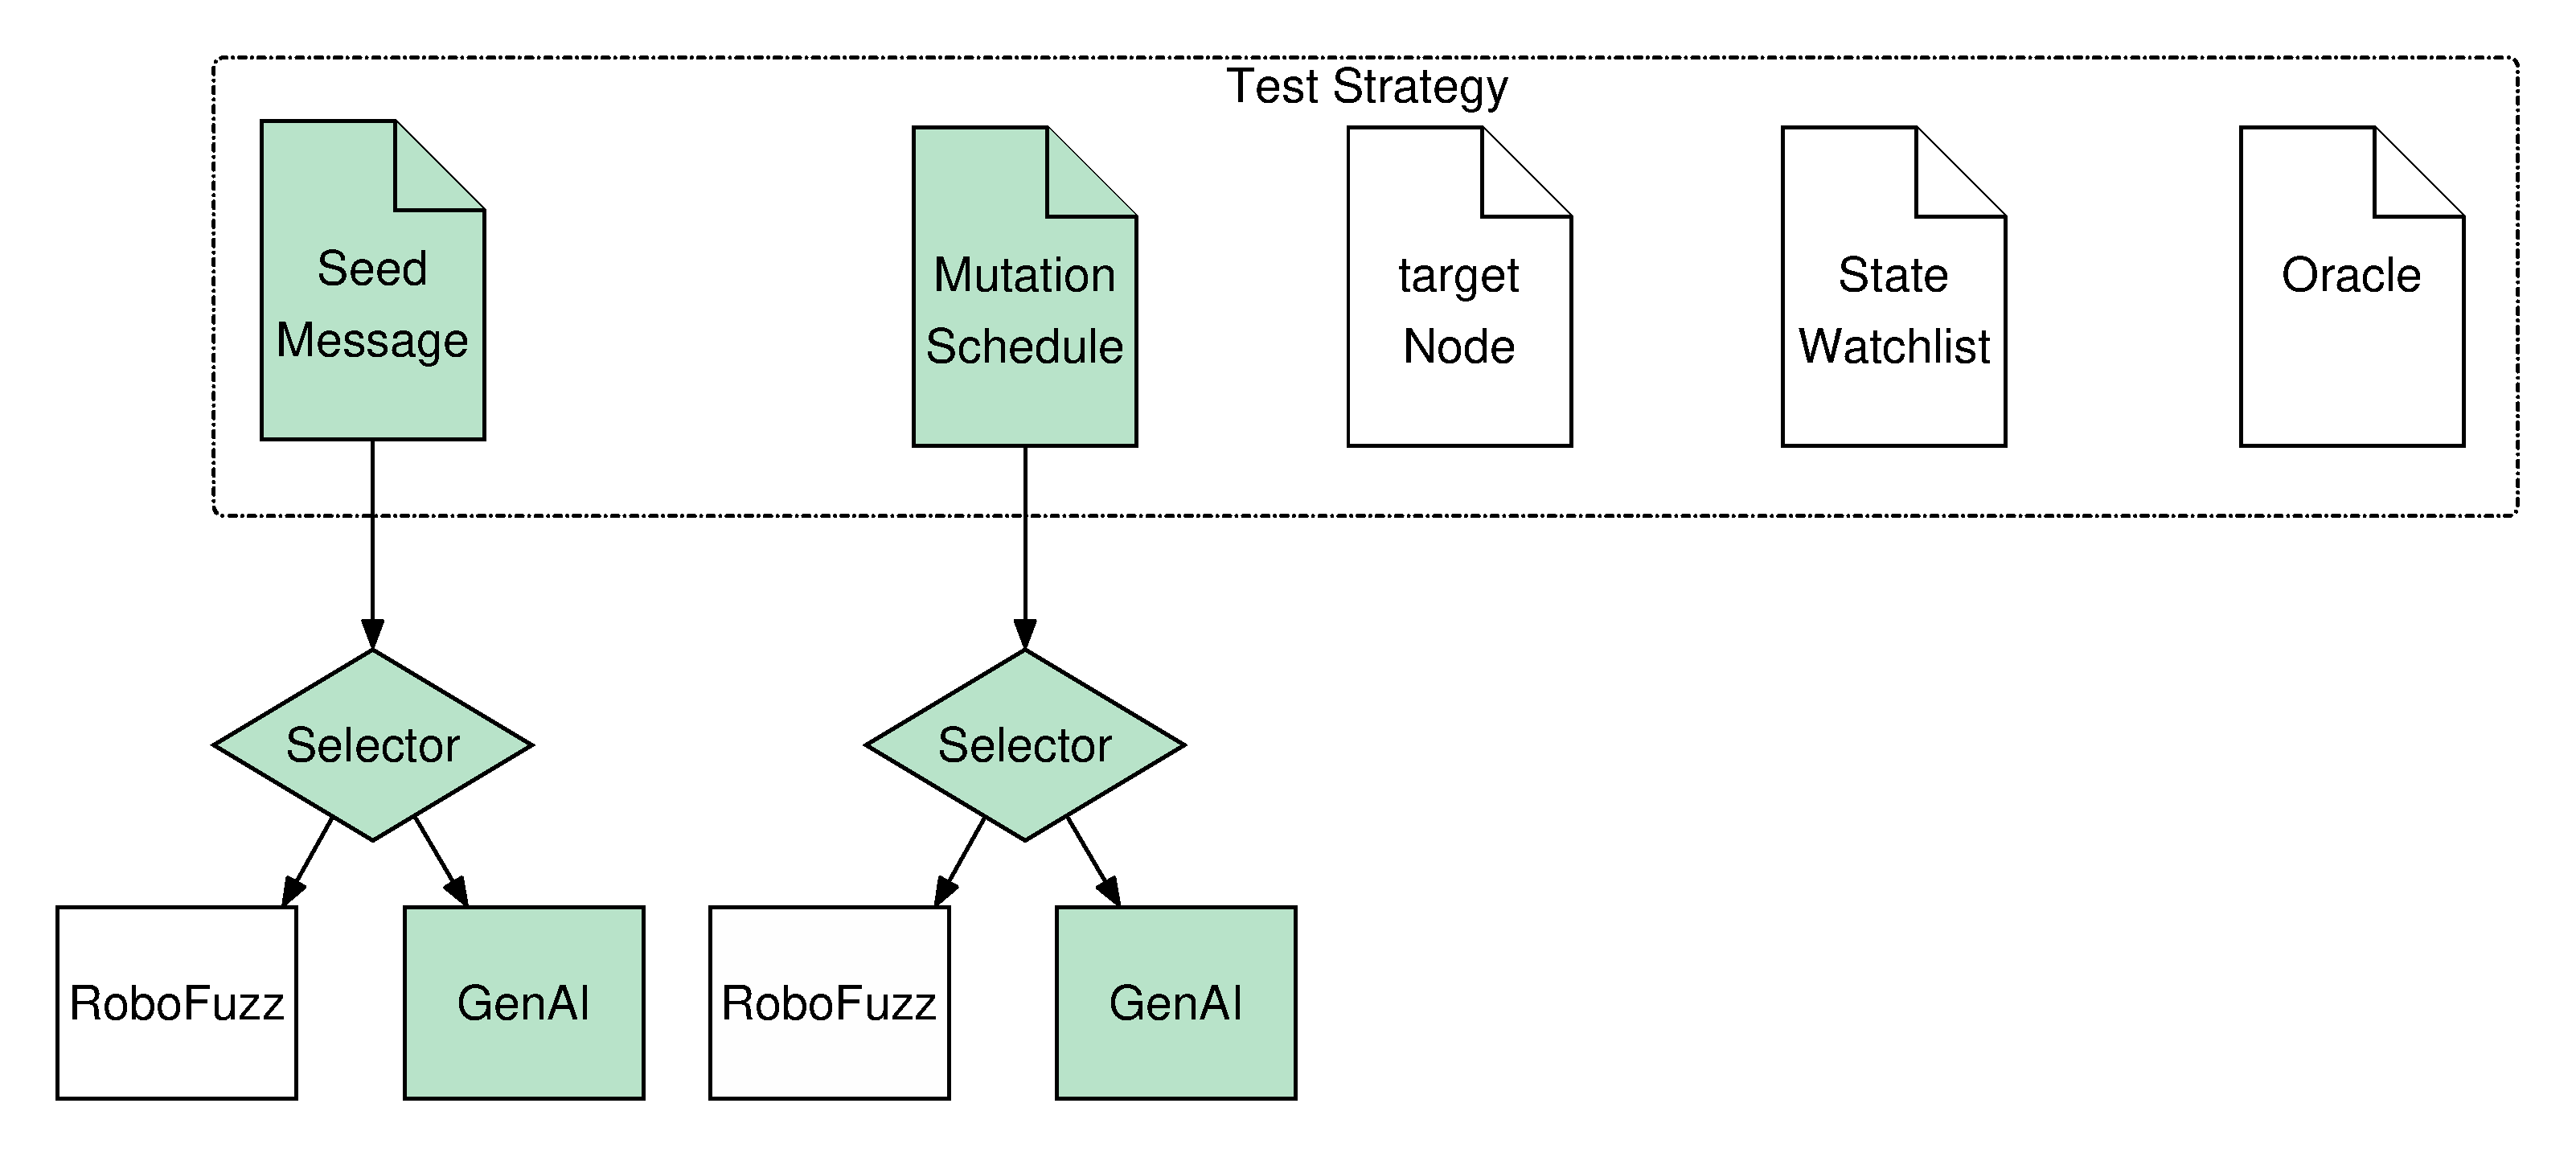
\includegraphics[width=0.7\linewidth]{ ./figures/data/Test_Strategy.pdf}}
    \caption{The input test strategies of RobotFuzz, inclusive of the genai module features.}
    \label{fig:genai-robofuzz_test_strategy}
\end{figure} 
\end{frame}

\subsection{Simulation}
\begin{frame}{Proof-of-Concept Design - Simulation}
 \textbf{Simulation with Turtlebot3(tb3) robot:} Conducted fuzzing on a differential wheeled mobile robot equipped with a LiDAR sensor designated topics.

%\SRC: https://robots.ros.org/assets/img/robots/turtlebot3/turtlebot3_series.png
\begin{figure}[ht!]
    \centering
    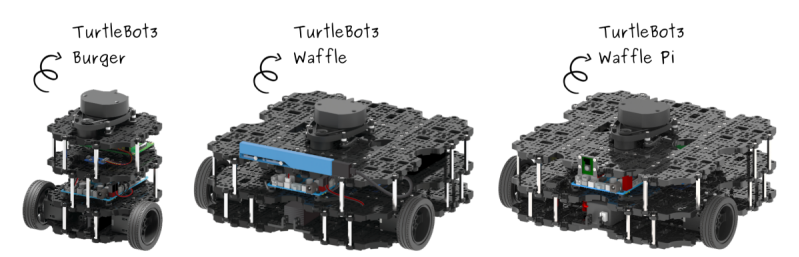
\includegraphics[width=1\textwidth]{./figures/data/turtlebot3_series.png}
    %\caption{TurtleBot version 3 series.}
    \label{fig:turtlebot3_series}
\end{figure}


\end{frame}

\subsection{Monitor}
\begin{frame}{Proof-of-Concept Design - Monitor}
\only<1>{
 %\textbf{Simulation with Turtlebot3(tb3) robot:} Conducted fuzzing on a differential wheeled mobile robot equipped with a LiDAR sensor designated topics.
 \textbf{rqt\_graph} associated all active nodes and topics during the validation process.

%\begin{figure}[htbp]
\begin{figure}[ht!]
    \centering
    \includesvg[width=0.6\textwidth]{./figures/data/rqt_graph/all/llama_ros-tb3.svg}
    \caption{rqt\_graph associated all active nodes and topics during the validation process.}
    \label{fig:robofuzz_rqt_graph_all_llama_ros-tb3}
\end{figure}
}

\only<2>{
%\begin{figure}[htbp]
\begin{figure}[ht!]
    \centering
    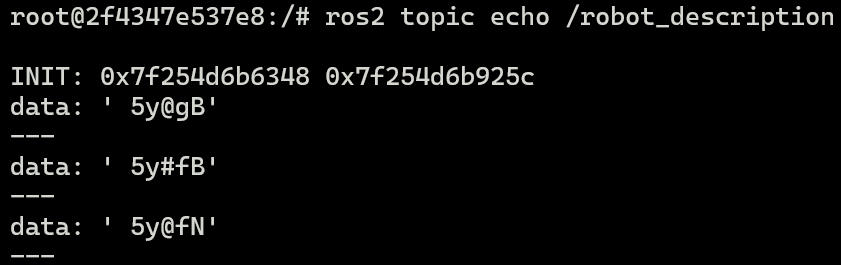
\includegraphics[width=0.5\textwidth]{./figures/data/ROS2_robot_description_echo.png}
    \caption{It shows the monitoring of messages received by the /robot\_description topic during the validation process.
}
    \label{fig:ROS2_robot_description_echo}
\end{figure}
}

\end{frame}

    

\subsection{Validation}
\begin{frame}{Proof-of-Concept Design - Validation}
 \textbf{Validation Process:} Detailed logs and statistics of the fuzzing process, including seed generation and mutation.
%%\begin{figure}[htbp]
\begin{figure}[ht!]
    \centering
    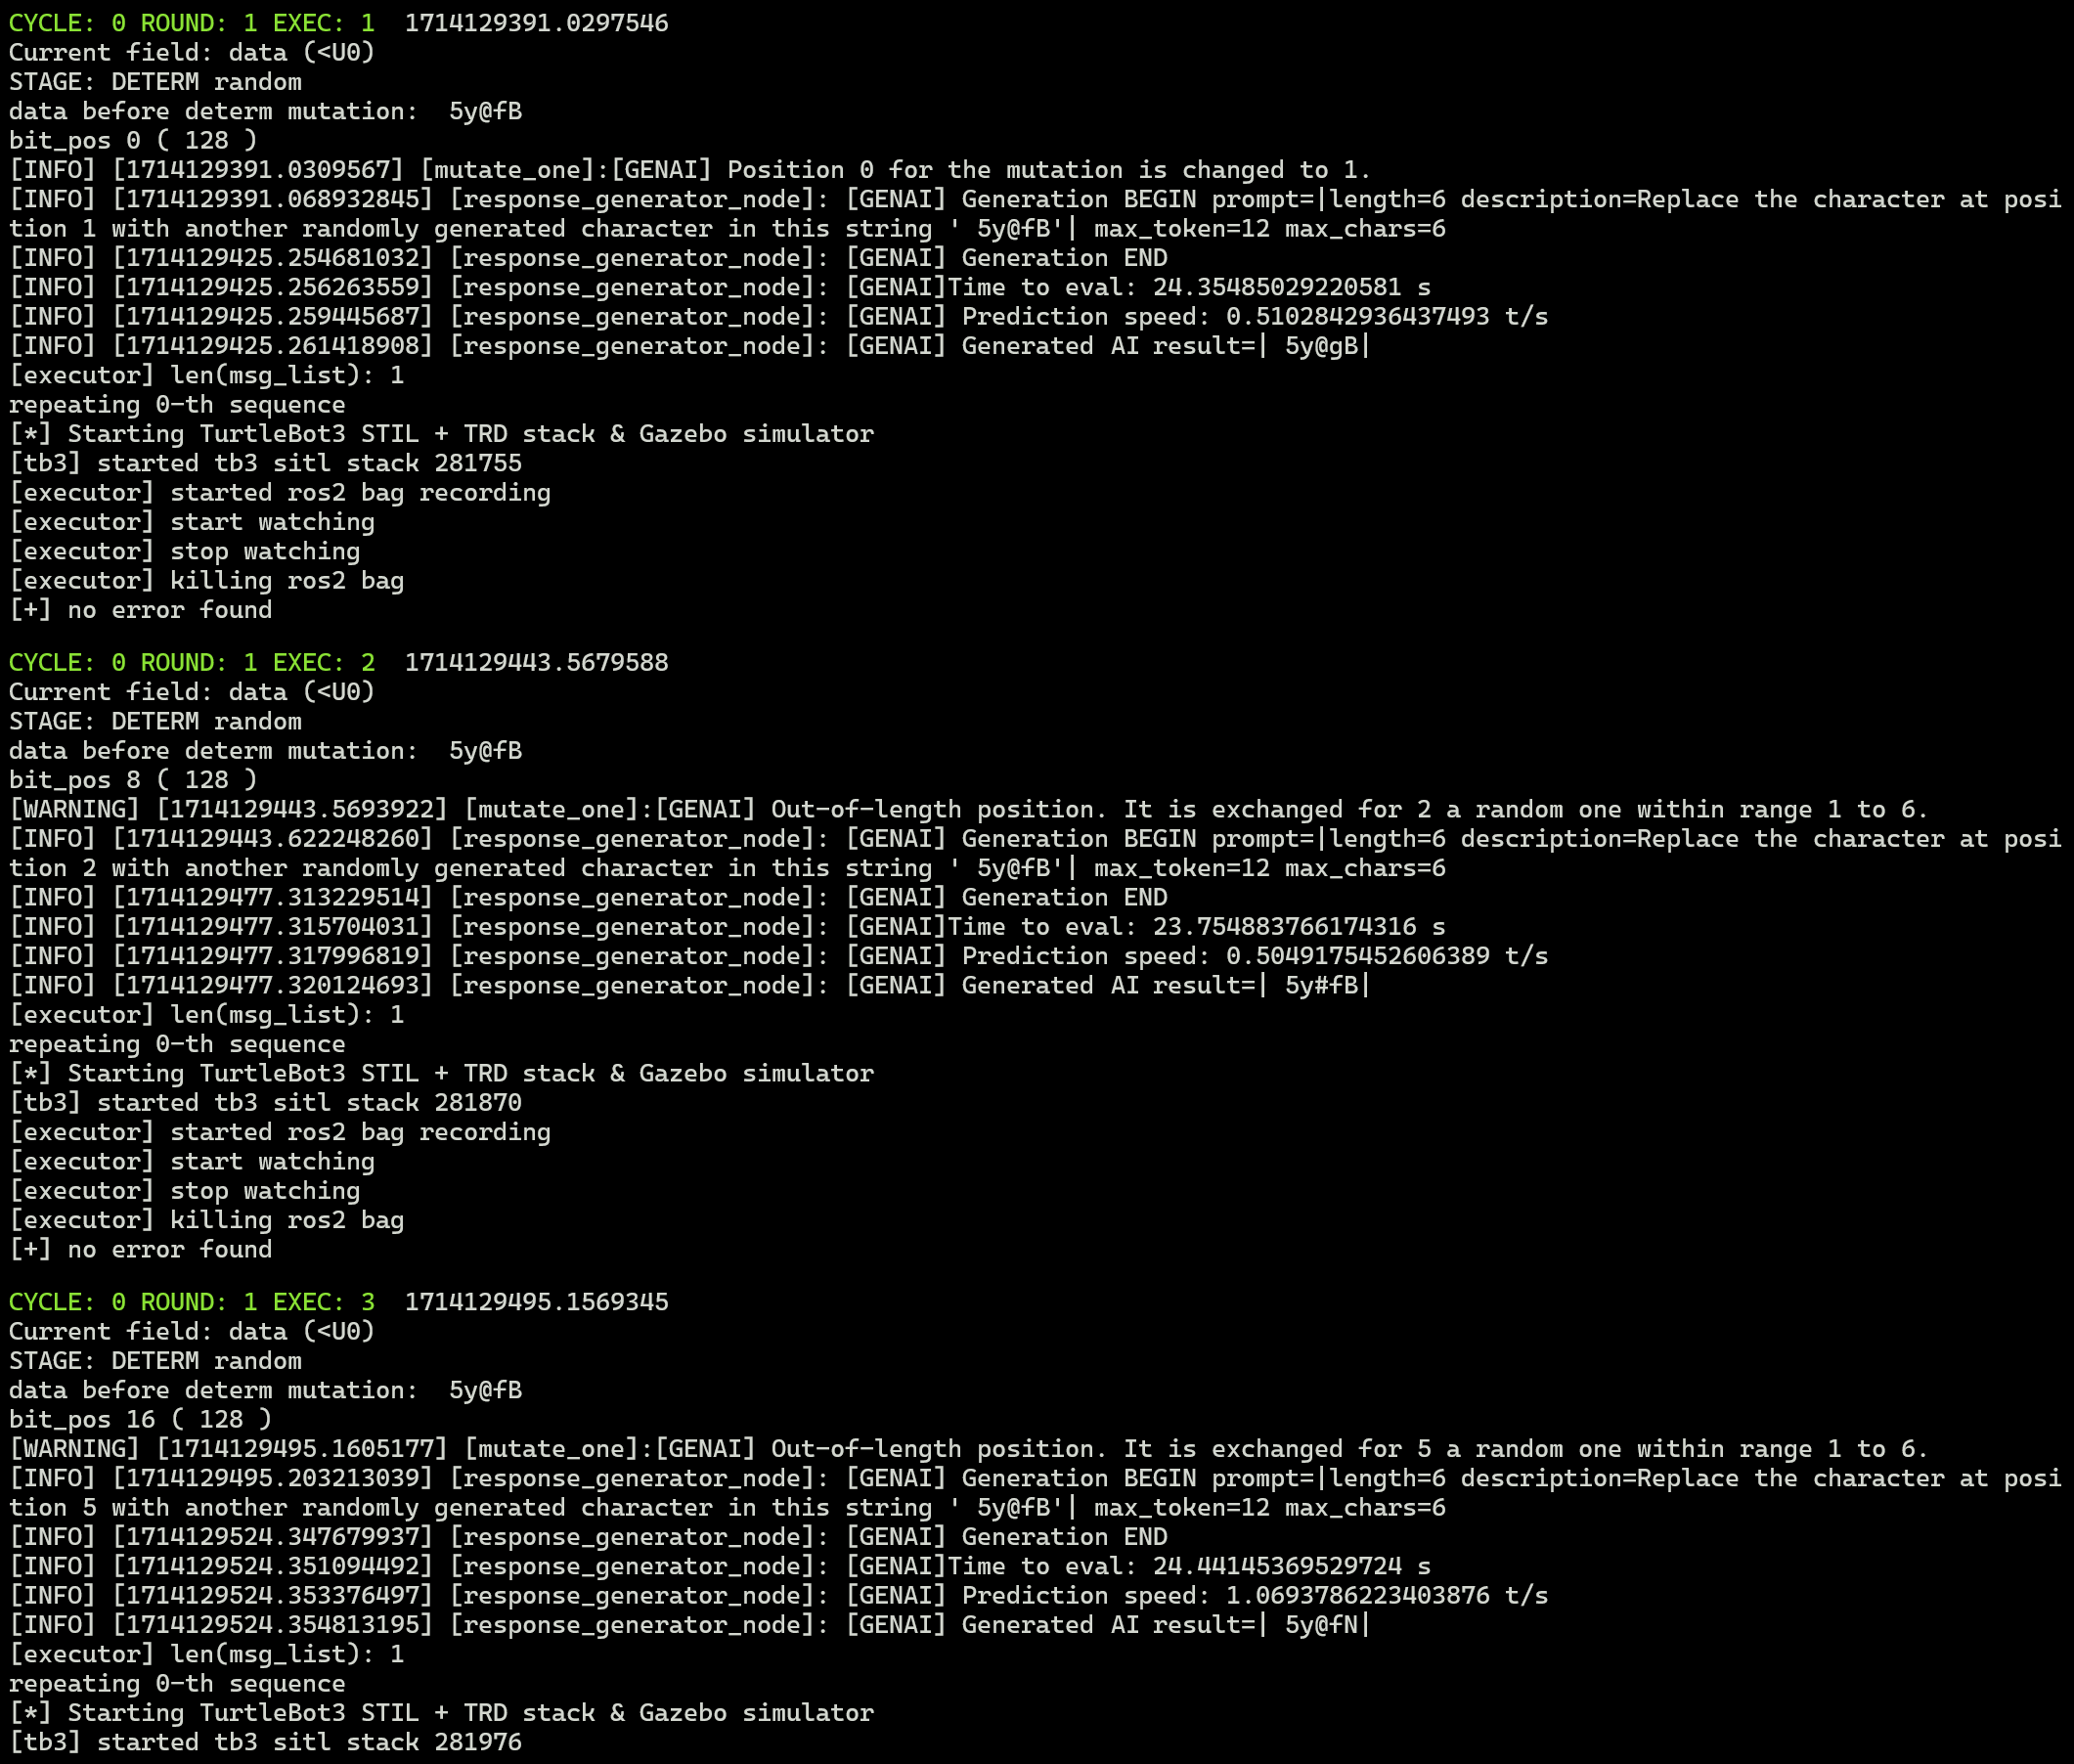
\includegraphics[width=1\textwidth]{./figures/data/robofuzz_genai_02_fase2_mutaciones.png}
    \caption{The operation of the GenAI module in mutation.}
    \label{fig:robofuzz_genai_02_fase2_mutaciones}
\end{figure} 


%\begin{figure}[htbp]
\begin{figure}[ht!]
    \centering
    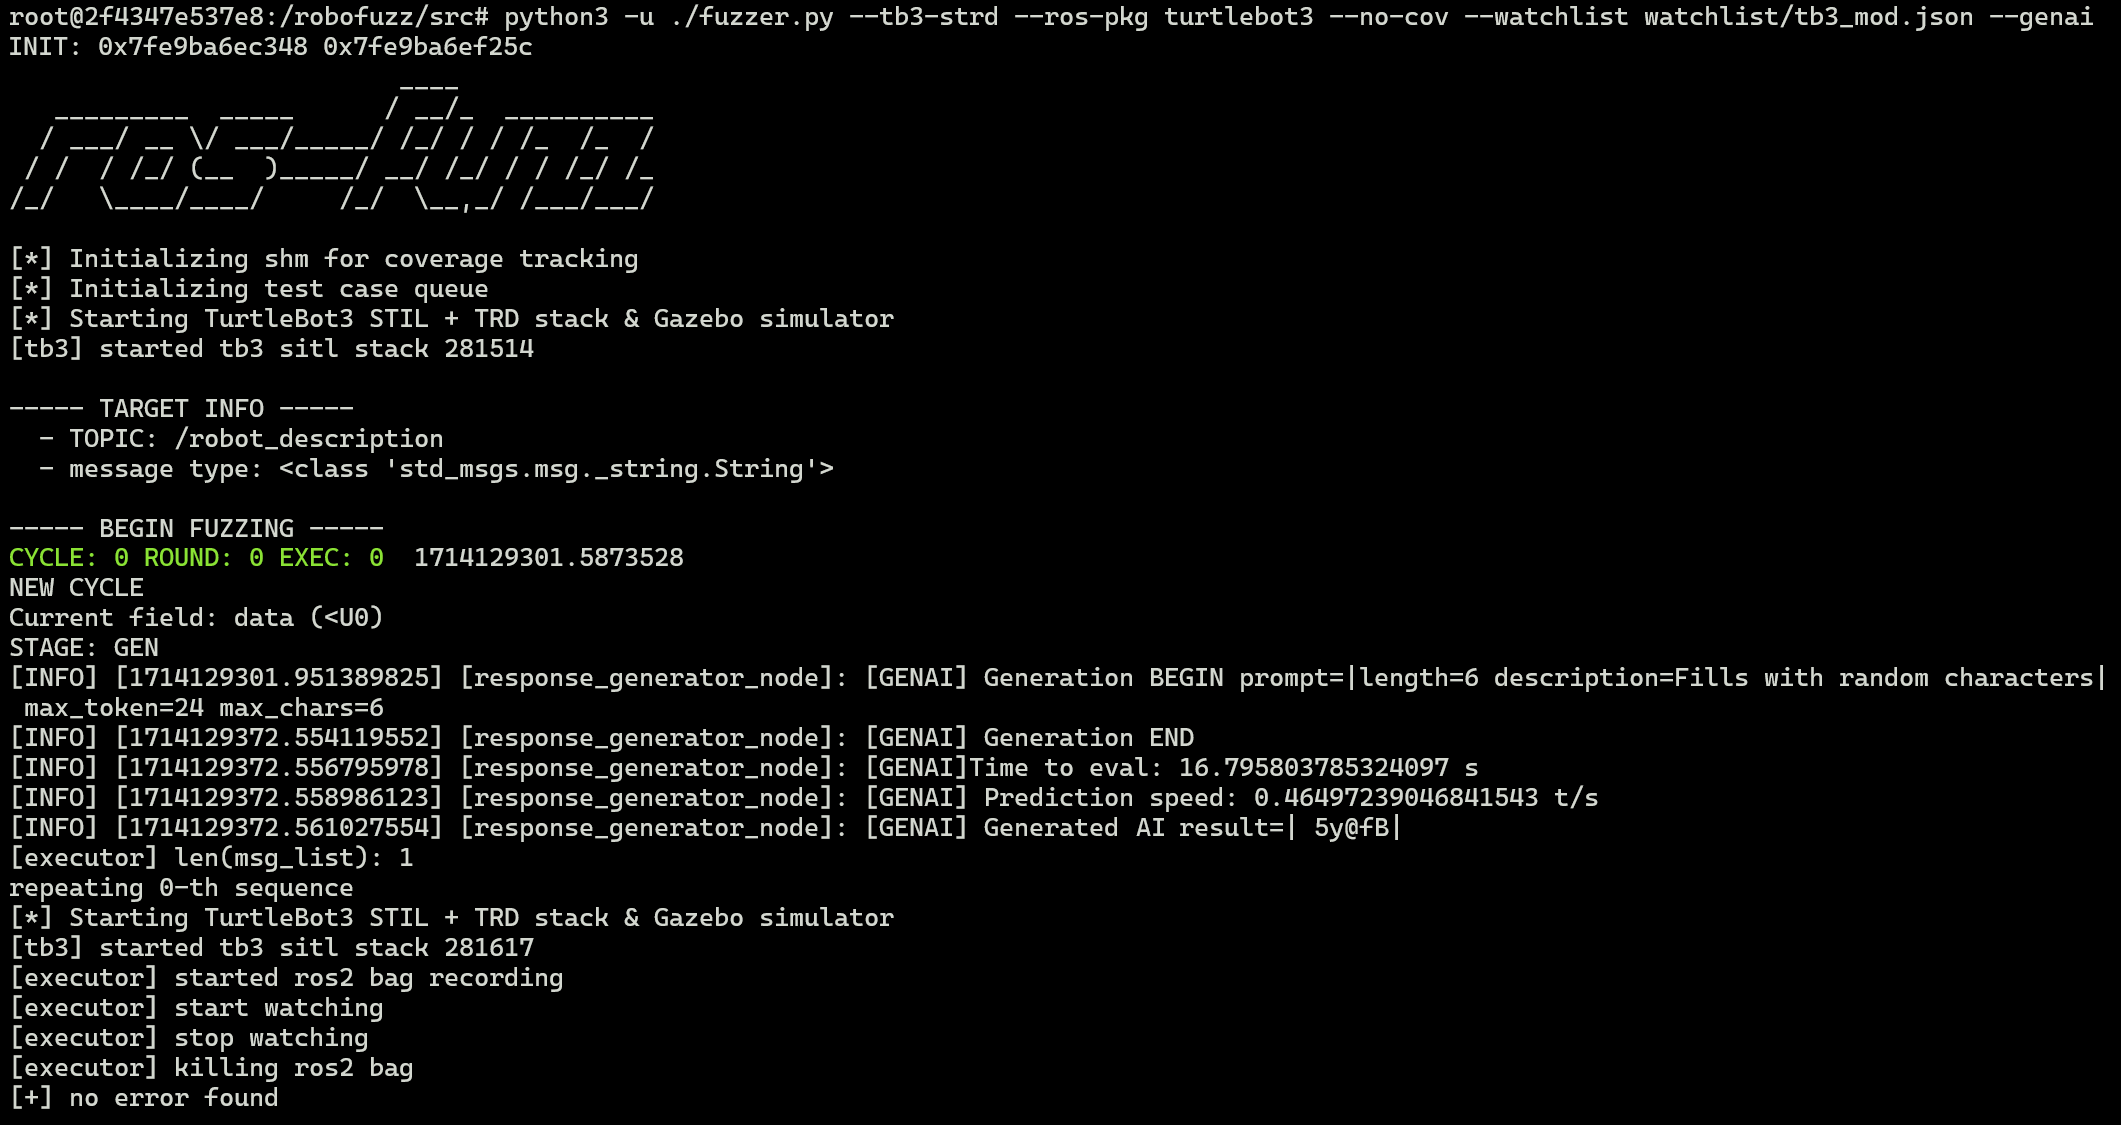
\includegraphics[width=1\textwidth]{./figures/data/robofuzz_genai_01_fase1_arranque+semilla_random.png}
    \caption{The operation of the GenAI module in seed generation.}    \label{fig:robofuzz_genai_01_fase1_arranque+semilla_random}
\end{figure}
\end{frame}

\begin{frame}{Proof-of-Concept Design - Validation}


%\begin{figure}[htbp]
\begin{figure}[ht!]
    \centering
    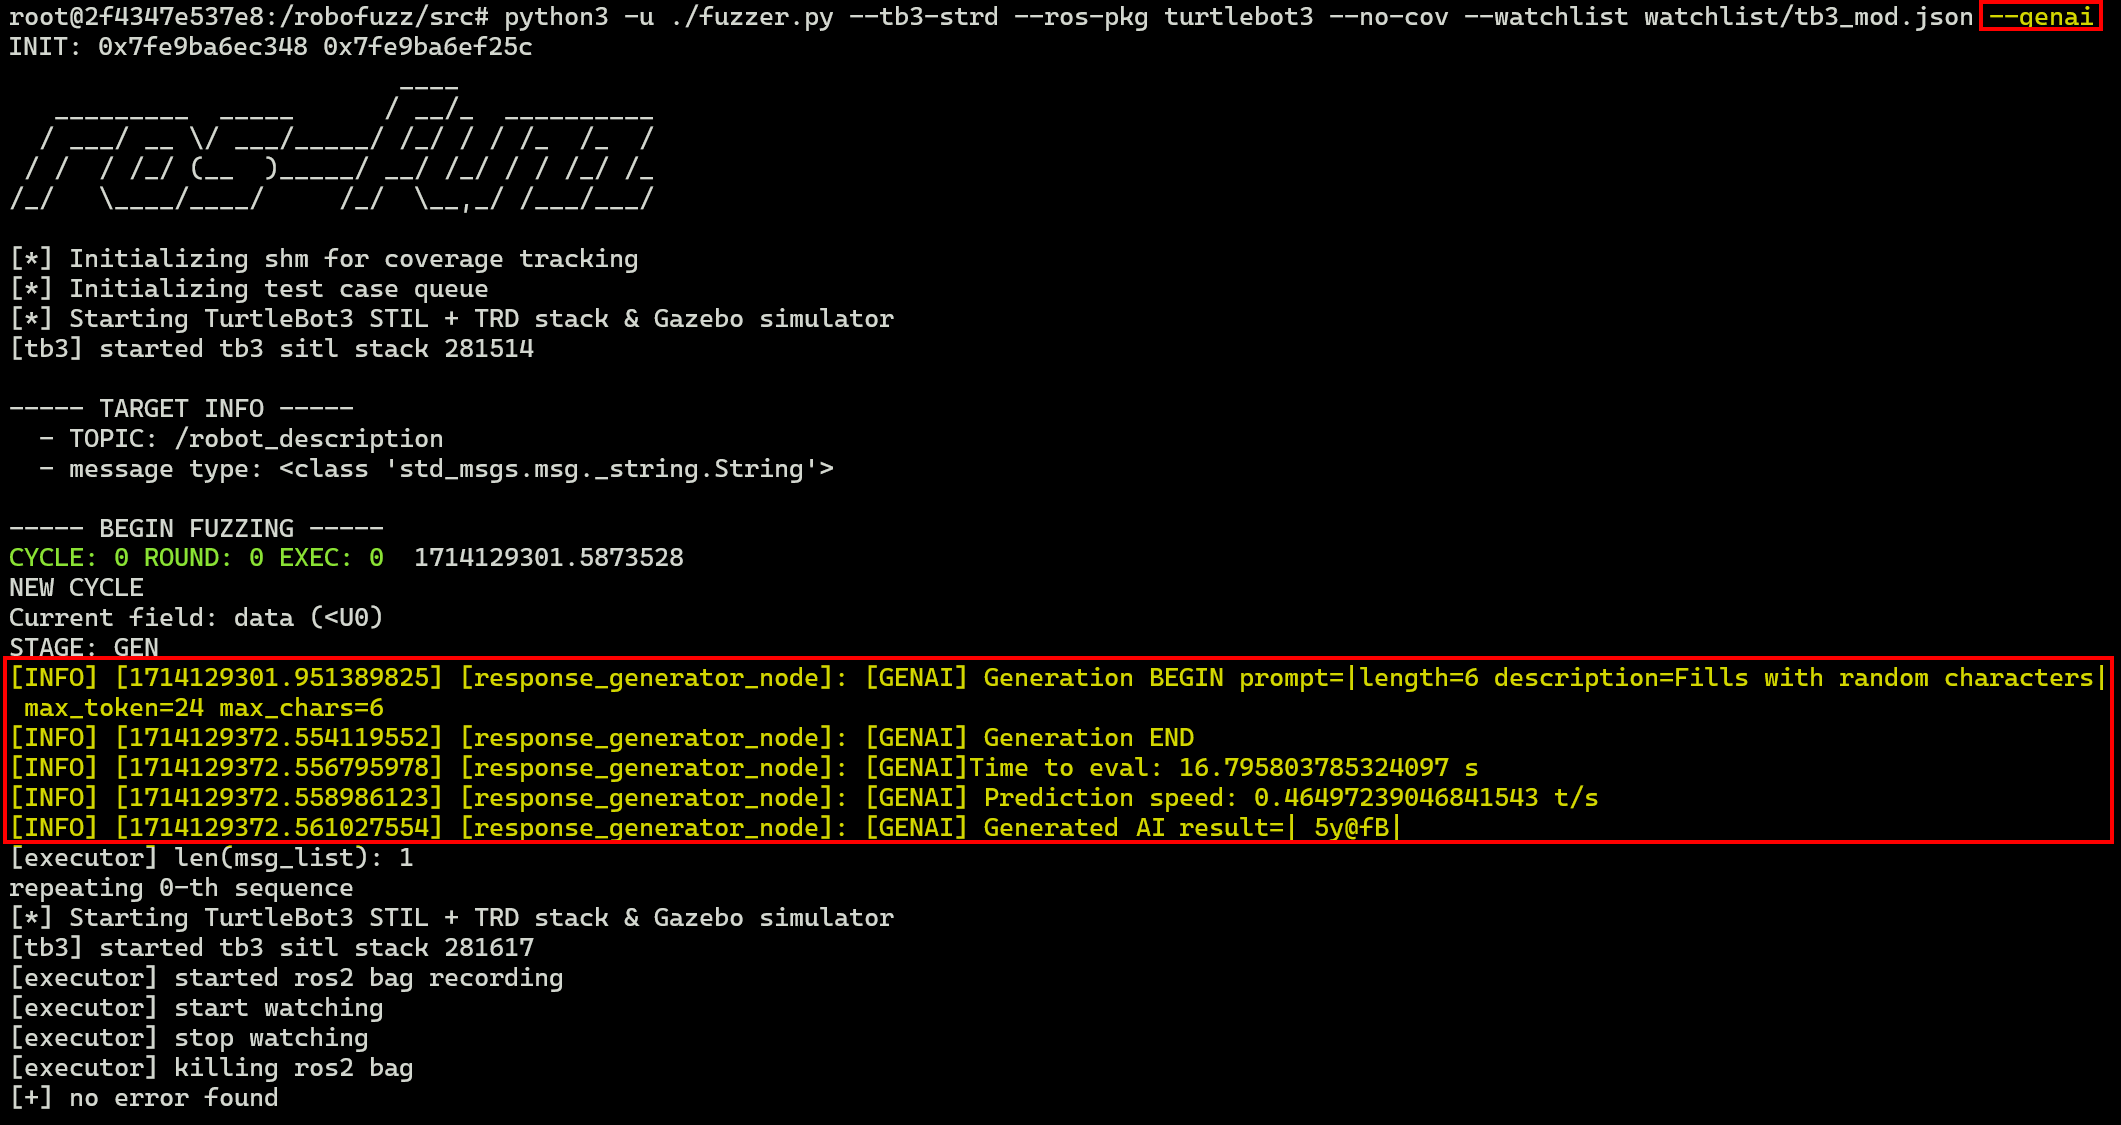
\includegraphics[width=1.0\textwidth]{./figures/data/robofuzz_genai_01A_RESALTADO_fase1_arranque+semilla_random.png}
    %\caption{The operation of the GenAI module in seed generation.}
    \label{fig:robofuzz_genai_01A_RESALTADO_fase1_arranque+semilla_random}
\end{figure}
\end{frame}


\section{Contribution}
\begin{frame}{Contribution}
\begin{tcolorbox}[drop shadow southeast, enhanced, colback=blue!5!white, colframe=Azuloscuro-cisis]
\begin{itemize}
    \item \textbf{Integration of LLM:} Developed a new module, GenAI, for RoboFuzz to utilize Large Language Models (LLM) in the seed generation and mutation process.
    \item \textbf{AI-Driven Fuzzing:} Replaced the traditional Mutator module with a generative AI model, enhancing the efficiency and effectiveness of fuzz testing.
    \item \textbf{Modular Design:} Designed for modular utilization with Singularity container technology, facilitating large-scale deployment in High-Performance Computing (HPC) environments.
    \item \textbf{Open Source Tool:} Provided a ready-to-use deployable tool with all associated materials, including the proof of concept and code, accessible on GitHub for review and utilization.
\end{itemize}
\end{tcolorbox}
\end{frame}

\begin{comment}
    
% Slide for Conclusions and Future Work
\section{Conclusions and Future Work}
\begin{frame}{Conclusions and Future Work}
\begin{tcolorbox}[drop shadow southeast, enhanced, colback=blue!5!white, colframe=Azuloscuro-cisis]
\begin{itemize}
    \item \textbf{Conclusions:}
    \begin{itemize}
        \item Demonstrated the viability and potential of integrating generative AI within an HPC environment for fuzz testing.
        \item Highlighted the benefits of using AI for automated input generation and mutation, improving the robustness and security of ROS2-based robotic systems.
    \end{itemize}
    \item \textbf{Future Work:}
    \begin{itemize}
        \item Explore the use of more specific AI models tailored for different tasks to enhance the quality of fuzz testing.
        \item Investigate the performance of AI-optimized hardware to improve the efficiency of generative AI models.
        \item Expand the application of the developed framework to other domains and robotic systems.
    \end{itemize}
\end{itemize}
\end{tcolorbox}
\end{frame}
\end{comment}

% Slide for Conclusions
\section{Conclusions \& Future Work}
\begin{frame}{Conclusions}
\begin{itemize}
    \item \textbf{Generative AI:}
    \begin{itemize}
        \item Represents a new paradigm with significant advantages, such as the ability to "program" generation and modification using natural language.
        \item Not always optimal for use cases that cannot be easily explained in natural language.
        \item Performance heavily depends on hardware characteristics, impacting efficiency on older or non-optimized systems.
    \end{itemize}
    \item \textbf{HPC Integration:}
    \begin{itemize}
        \item Enhances the effectiveness and efficiency of fuzz testing techniques for ROS2 robotic systems.
        \item Contributes to the reliability and security of ROS2 systems by enabling parallelization and acceleration of the fuzz testing process.
    \end{itemize}
\end{itemize}
\end{frame}


% Slide for Future Work
%\section{Future Work}
\begin{frame}{Future Work}
\begin{tcolorbox}[drop shadow southeast, enhanced, colback=blue!5!white, colframe=Azuloscuro-cisis]
\begin{itemize}
    \begin{itemize}
        \item \textbf{Specific AI Models:} Explore the use of more specific AI models tailored for different tasks to enhance the quality of fuzz testing. This includes developing models that can handle specific types of data or scenarios encountered in ROS2 systems.
        \item \textbf{AI-Optimized Hardware:} Investigate the performance of AI-optimized hardware to improve the efficiency of generative AI models. This involves testing on newer hardware with better support for AI workloads to reduce latency and increase throughput.
        \item \textbf{Framework Expansion:} Expand the application of the developed framework to other domains and robotic systems. This could involve adapting the framework for use in different types of robots or in other areas of software testing.
        \item \textbf{Integration with Other Tools:} Integrate the fuzzing framework with other security and testing tools to create a more comprehensive testing suite.
    \end{itemize}
\end{itemize}
\end{tcolorbox}
\end{frame}


% PREGUNTAS %%%%%%%%%%%%%%%%%%%%%%%%%%%%%%%%%%%%%

\begin{frame}
%\begin{frame}[plain,standout]
\begin{center}
\vspace*{\stretch{0}}
{\centering\Huge\textcolor{black!50}{Thank you for your attention.}\par Do you have any questions?}%
\vspace*{\stretch{9}}

%\centering

\includegraphics[width=0.9\textwidth]{./img/mecenas_logos.png}

\end{center}
    
\end{frame}

%\titleframe
%\appendix

% REFERENCIAS %%%%%%%%%%%%%%%%%%%%%%%%%%%%%%%%%%%%%
%
%\begin{frame}[allowframebreaks]{References}
%
%    \bibliographystyle{spmpsci}
%    \bibliography{bibliography.bib}
%
%\end{frame}


\end{document}

